\chapter{Experimentos}
\label{cap:experimentos}

Como se ha comentado en el apartado del estado del arte, la investigación acerca de este tema sigue en curso y todavía no hay una solución generalista para reemplazar los solvers físicos con modelos de Machine Learning. Utilizando la infraestructura descrita en el capítulo anterior, se ha comparado la efectividad de modelos con diferentes características, con el fin de analizar las limitaciones de esta alternativa y descubrir que técnicas resultan ser más prometedoras. \newline

A la hora de valorar la calidad de un sistema de inferencia en tiempo de ejecución, hay dos criterios fundamentales:
\begin{itemize}
  \item \textit{Resultado visual}: El movimiento inferido por el modelo ha de respetar las reglas fisicas suficientes para tener credibilidad. Además, es importante que la simulación se mantenga estable y la tela mantenga su estructura a lo largo de la ejecución.
  \item \textit{Rendimiento}: Los modelos deben ser capaces de competir con los reducidos tiempos de computo de los solvers. Para ello tanto los modelos como los datos de input han de ser lo más ligeros posibles.
\end{itemize}

A lo largo del proyecto se han llevado a cabo numerosas pruebas, a continuación se describen los experimentos con los resultados más interesantes. Pueden verse de forma interactiva en la aplicación del repositorio.

\section{Recurrencia}


Los siguientes parámetros son compartidos entre ambas pruebas, con la intención de aislar únicamente la recurrencia y analizar su efecto.
\begin{table}[H]
    \begin{center}
        \begin{tabular}{ | m{2.2cm} | m{2cm} | m{1.2cm} | m{2.1cm} | m{2.4cm} | m{2.2cm} | }
        \hline \textbf{Windows size} & \textbf{Rollout steps} & \textbf{Noise} & \textbf{Learning rate} & \textbf{Tamaño dataset} & \textbf{Batch size} \\ \hline
            16 & 24 & 3\% & 0.001 & 25000 & 32 \\ \hline
        \end{tabular}
            \end{center}
    \caption{Hiperparámetros y configuración del entrenamiento.}
    \label{tab:randomTraining}
\end{table}

\begin{table}[H]
    \begin{center}
        \begin{tabular}{ | m{3cm} | m{3cm} | m{3cm} | m{1.2cm} | m{2cm} | }
        \hline \textbf{Prueba} & \textbf{Tiempo} & \textbf{Error medio por vertice} & \textbf{FPS} & \textbf{Percepción} \\ \hline
            MLP & 20h(gpu) & 0.000923 & 110 & 8/10 \\ \hline
            RNN & 20h(gpu) & 0.000923 & 110 & 8/10 \\ \hline
        \end{tabular}
    \end{center}
    \caption{Resultados del entrenamiento.}
    \label{tab:randomResults}
\end{table}


\section{Velocidad}
Como se ha mencionado anteriormente, hay varias características que se registran en la fase de simulación, de las cuales algunas han resultado ser más óptimas para generar un entrenamiento ligero y efectivo: la posición de los vértices, la velocidad y el sdf. Al utilizar secuencias de frames para el entrenamiento, la velocidad puede ser redundante, por lo que en este experimento se valora su efecto.

Hay que calcular la velocidad de cada punto de la tela en cada frame para generar el tensor de entrada. Además del coste computacional que esto supone, el ERROR de ...


\section{PCA}
Siguiendo con la noción de disminuir la ......

A la hora de escalar el proyecto, aumentando tanto la geometría como los tipos de movimiento, resulta interesante introducir un modelo que se valga de un PCA para reducir la dimensión de los parámetros de entrada. Utilizando el método del umbral de varianza, se calcula el mínimo de características necesarias para alcanzar un gran porcentaje de la variabilidad de los datos. En el caso de la figura por ejemplo, partiendo de un dataset con 25 vértices y 13 features por cada uno, que resultaría en 325 elementos de input, con un umbral de varianza del 95\% consigue reducirse a 45. 


\section{Unrolling}
De manera similar, en este proyecto se genera una secuencia de predicciones; la cadena de deltas generados sucesivamente permiten al modelo tener una noción sobre el cambio de velocidad y aceleración provocados. Esta técnica consiste en retropropagar el error a lo largo de la secuencia temporal y permite a la red aprender dependencias temporales.





%\subsection{Gestión del error acumulado}
%En este punto del desarrollo, los resultados de accuracy del modelo son adecuados, se alcanzan entrenamientos con un error medio por vertice de hasta 0.001m, lo que en un contexto estático sería imperceptible. Sin embargo, nuestro modelo ha de mantenerse consistente a lo largo del tiempo. A 60 fotogramas por segundo, un error tan bajo puede convertirse en una geometría completamente dañada al cabo de pocos segundos. Ante este problema, se plantean varias opciones para que el aprendizaje pueda ser capaz de autocorregirse.

%\begin{figure}[H]
%        \centering
%        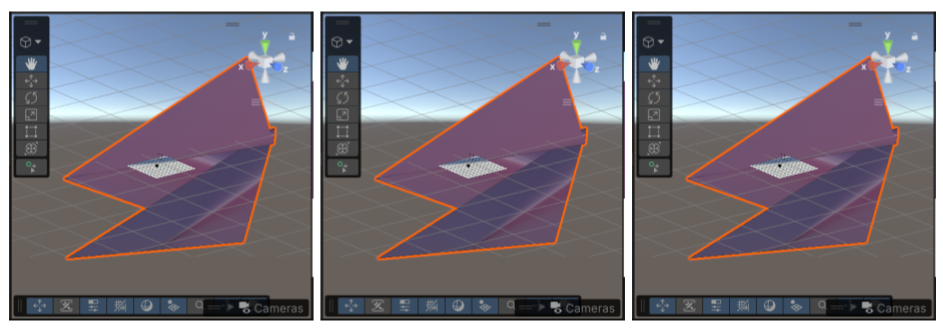
\includegraphics[width=0.91\textwidth]{Imagenes/errorAcumulado.png}
%        \caption{Reducción de características}
%    \end{figure}

%\textbf{Anchored training:} Otra forma de intentar reducir el error consiste en inferir el desplazamiento de los vértices respecto a las posiciones originales de la malla en lugar de las posiciones en el último frame (\cite{bertiche_deepsd_2021}, \cite{santesteban2022snug}, \cite{holden_subspace_2019}). Este es un planteamiento intuitivo que se presenta en distintos papers mencionados previamente: DeePSD, SNUG o Subspace Neural Physics. Al pensar en simulaciones de telas, ya sea una bandera con su mástil o una prenda con su personaje, todas cuentan con unos puntos, es decir, algo a lo que anclarse. Actuando sobre esos puntos se puede asegurar que la simulación se mantendrá dentro de un espacio concreto. En esta investigación aplicamos esta técnica guardando las posiciones de los vértices en su estado incial y aplicando los nuevos desplazamientos sobre estos.
%Al coger un punto de referencia del que medir los desplazamientos y no basarse en posicines generadas, el MSE del modelo, calculado como la diferencia entre las posiciones reales y predichas, en las pruebas de python mejora notablemente. No obstante, la simualción en Unity aún adolece de errores de pecisión.